\section{Why naïve globalization fails}
\label{sec:failed-shortcuts}

The preceding results reduce arbitrary curved data to finitely many polytopes and finitely many whole-word repair patches.  The final step is not automatic.  This section gives an exact rational calibration showing why repairs must be synchronized by complete words.

\begin{example}[Sequential repair can recreate a forbidden word]
\label{ex:sequential-failure}
Work in the open square $X=(-3,3)^2$.  The source fields are
\[
 U_1=U_3=X,
\]
and $U_2$ is the interior of
\[
 P_2=\conv\{(0,-1),(1,1/10),(2,1/10),(2,-1/10)\}.
\]
The covered source code is
\[
 \C=\{13,123\}.
\]
Let
\[
 P_3^0=[-2,2]\times[-1/10,1/10]
\]
and
\[
 P_1^0=\conv\{(-2,-1/10),(2,-1/10),(2,1/10),(0,1),(-2,1/10)\}.
\]
The points
\[
 (-3/2,0)\in A_{13},
 \qquad
 (3/2,0)\in A_{123}
\]
are protected target witnesses.  The tuple also realizes forbidden words: $(0,4/5)$ has word $1$, and $(1/5,-4/5)$ has word $2$.

First replace $P_3^0$ by $P_1^0$.  Then every membership in neuron $1$ is accompanied by neuron $3$, so words $1$ and $12$ disappear.

Next attempt to repair word $2$ using neuron $1$ alone.  Replace $P_1^0$ by
\[
 P^{\rm hull}=\conv(P_1^0\cup P_2).
\]
The exact point
\[
 q=(-1,-3/10)
\]
lies in $\operatorname{int}P^{\rm hull}$ but outside both $P_2$ and the unchanged $P_3=P_1^0$.  Hence the forbidden word $1$ reappears.

In contrast, the synchronized replacement
\[
 P_1=P_3=P^{\rm hull}
\]
realizes exactly $\{13,123\}$ on $\operatorname{int}P^{\rm hull}$: points outside $P_2$ have word $13$, and points inside $P_2$ have word $123$.
\end{example}

\begin{figure}[t]
\centering
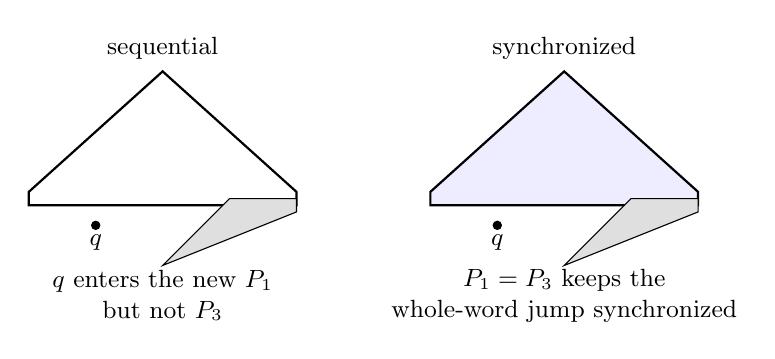
\begin{tikzpicture}[scale=.85,font=\small]
\begin{scope}
\draw[thick] (-2,0)--(2,0)--(2,.2)--(0,2)--(-2,.2)--cycle;
\draw[fill=gray!25] (0,-.9)--(1,.1)--(2,.1)--(2,-.1)--cycle;
\fill (-1,-.3) circle (2pt) node[below]{$q$};
\node at (0,2.35) {sequential};
\node[align=center] at (0,-1.35) {$q$ enters the new $P_1$\\but not $P_3$};
\end{scope}
\begin{scope}[xshift=6cm]
\draw[thick,fill=blue!7] (-2,0)--(2,0)--(2,.2)--(0,2)--(-2,.2)--cycle;
\draw[fill=gray!25] (0,-.9)--(1,.1)--(2,.1)--(2,-.1)--cycle;
\fill (-1,-.3) circle (2pt) node[below]{$q$};
\node at (0,2.35) {synchronized};
\node[align=center] at (0,-1.35) {$P_1=P_3$ keeps the\\whole-word jump synchronized};
\end{scope}
\end{tikzpicture}
\caption{Sequential versus synchronized repair in \Cref{ex:sequential-failure}.  Enlarging neuron $1$ alone creates a remote $1$-atom; enlarging neurons $1$ and $3$ by the same whole-word hull preserves their synchronized activity.}
\label{fig:sequential-failure}
\end{figure}

\begin{proposition}[The finite compatibility problem is genuine]
The atlas of \Cref{thm:repair-atlas} cannot in general be globalized by a fixed ordering of independent per-neuron convex-hull enlargements.  Even when every patch is source-contained and every target witness is protected, a later enlargement may create a forbidden atom outside the patch that motivated it.
\end{proposition}

\begin{proof}
The first repair in \Cref{ex:sequential-failure} removes the forbidden word $1$.  The second enlargement is source-contained, repairs a different current defect, and nevertheless creates a new $1$-atom at the rational point $q$.  Thus neither source containment nor monotone enlargement gives global monotonicity of the atom code.
\end{proof}

\subsection{A sharper one-round failure}

For completeness, the reproducibility package also includes a three-neuron example with source code
\[
 \{\varnothing,1,2,123\}
\]
in which a single $123$-patch covers the entire old $12$-carrier, is added simultaneously to all three neurons, and yet a remote rational point still has word $12$.  A second larger common-core patch removes the circuit.  This example shows that ``add every patch to every neuron in its label in one round'' is also not a theorem.  We keep it in the appendix because the simpler sequential example already isolates the conceptual issue.

\subsection{Other shortcuts ruled out}

Three additional cautions delimit the scope of our results.

\begin{enumerate}[label=\textup{(\roman*)}]
\item \textbf{Nerve preservation is insufficient.}  A nerve-preserving approximation may expose a smaller atom, even when every intersection remains nonempty.
\item \textbf{Witness preservation is insufficient.}  Keeping one point from every target atom proves only $\C\subseteq\D$; it does not rule out $\D\setminus\C$.
\item \textbf{Intersection completion is not a retract shortcut.}  A surjective image of an intersection-complete code is intersection complete \cite[Theorem~1.5]{Jeffs2020}.  Therefore a non-intersection-complete code cannot be obtained as a morphic retract of its intersection completion; see \Cref{app:intersection-morphisms}.
\end{enumerate}

The remaining task is neither uncontrolled approximation nor an infinite local repair problem.  It is a finite global compatibility problem: attach a finite collection of whole-word modules while each original neuron is represented by one convex polytope and no mixed convex combination produces a forbidden intermediate word.
